\documentclass{article}
\usepackage{graphicx}
\usepackage{listings}
\usepackage{url}
\title{An Investigation of Lesser Known Programming Languages}
\author{David Colgan}
\date{\today}
\begin{document}
\maketitle

\tableofcontents

\begin{abstract}
%%%talke about how my program is more complicated than prechelt's

In the software industry today most systems are implemented with a C-like,
imperative or object-oriented language.  Many functional languages claim to
improve programmer productivity with higher expressiveness and safety,
resulting in shorter programs and fewer bugs.

Are these claims justified?  Anyone can claim that their favorite language is
the best.  This project seeks to verify these claims of shorter programs and
higher safety by systematically comparing C and Python, two commonly used
languages, with Clojure, Haskell, and Factor, three lesser known languages.

After studying them to be able to produce as idiomatic code as possible, I
write a simulator of the dice game Farkle in each language.  I then compare the
languages feature-by-feature and by comparing the source of each program, the
two approaches most commonly employed in the literature.

In the end, I agree with the advocates of these languages -- Clojure, Haskell,
and Factor offer compelling reasons for their use over C and Python.  The
functional languages have unique features like immutable variables,
higher-order functions, extensive type systems, macros, and laziness that allow
them to save the programmer time and effort.  I also am able to write a Farkle
simulator in fewer lines of code.  The Clojure simulator is just under half as
long as the C implementation, and the others come out similarly.

Further study is needed, but the savings in program size and programmer
efficiency of powerful functional languages look to revolutionize the software
development industry.  The 

\end{abstract}

\section{Introduction}

Most computer science majors and software developers have used Java and C.
According to the TIOBE Index~\cite{tiobe}, these two languages have
consistently been among the most popular for general use.  They are both
established, well understood, and use the object-oriented or imperative
paradigm.

Most of the other top languages are similar to Java and C.  Languages
like C\#, PHP, Python, Perl, and Objective-C all use some combination of the
procedural and object-oriented paradigm.   But are procedural and object
oriented languages the best computer science has to offer for creating
reliable, high performing software on a budget?

A number of lesser-known languages, many influenced by the functional
paradigm, claim increased programmer productivity, fewer bugs, and shorter
programs.

\section{Research Goals}

This project investigates languages that have the potential to be
compelling alternatives to the common procedural and object-oriented languages
most often used today in commercial environments.  I want to know if they live
up to the hype generated by their communities.

In the two semesters of this project I investigated three lesser-known
languages and two common languages as a comparison.  The two common languages
are C and Python, and the three lesser-known languages are Clojure, Haskell,
and Factor.  

\section{Literature Survey of Previous Work}
\label{sec:survey}

Two kinds of research in the literature compare programming languages:
feature-by-feature comparisons and comparisons of small programs.

\subsection{Feature Comparisons}

Feuer and Gehani~\cite{FeuerCVsPascal} take a conceptual approach when they compare C and
Pascal.  They begin with a history of the languages and
discuss design decisions, followed by a step-by-step walk through each
language's major features.  They also evaluate C and Pascal for different
problem domains.  This paper is more of an informative overview than a hard
empirical evaluation.  The only actual code they show is a single function
implementing binary search.

In a comparison of Ada 95 and Java, Brosgol~\cite{BrosgolCompOOAdaVsJava} takes
a similar approach, going feature-by-feature through the two languages.  He
provides sample code snippets throughout.  He arrives at a table of features,
highlighting differences in syntax, program organization features, memory
management, and OO features like inheritance, polymorphism, and encapsulation.

Nami~\cite{NamiCompOOSoftEng} presents a factual comparison of Eiffel, C++, Java, and
Smalltalk.  He gives a brief introduction to each
language, describing design decisions and history.  He then classifies each
language based on static vs.~dynamic typing, compiled vs.~interpreted build
methods, built-in quality assurance facilities, automatic documentation
generators, multiple vs.~single inheritance, and concludes with a brief
discussion on each language's efficacy for building infrastructure.

Tang~\cite{TangAdaVsCpp} does a similar comparison of Ada and C++ using many of
the same methods as the other studies.

Many of these studies are a high level overview of various languages.  They
compare features, but do not give in-depth examples.

\subsection{Program Comparisons}

Perhaps more useful and interesting are those comparisons done by inspecting
the same program written in different languages.  These give concrete examples
of the differences between languages.

The method I follow for this project is closely related to the method used by
Prechelt~\cite{Prechelt7LangComp}.  He compares C, C++, Java, Perl, Python,
Rexx, and Tcl by having various computer science masters students and
volunteers from newsgroups write the same small program in one of the
languages.  He then compared the programs based on program execution
time, memory consumption, lines of code, program reliability (based on whether
the program crashes or not), the amount of time it took each programmer to
write the program, and program structure.  The program he had the participants
write was a simple string processing program that consisted of converting
telephone numbers into sentences based on a large dictionary and mapping
scheme.  Most of the programs he received were fairly small, taking a median of
3.1 hours to write, and averaging 200-300 line of code.

Some of the more interesting results from Prechelt's study include the
observation that in lower-level languages, a lot of code is dedicated to
writing the data structures, while the higher-level languages, the programmer
usually takes advantage of the language's built-in capabilities.  He also found
that the scripting languages (Perl, Python, Rexx, and Tcl) tend to require
about twice as much memory as C and C++, with Java taking 3--4 times as much,
and that C and C++ are about twice as fast as Java and several times faster
still than the scripting languages.

Prechelt discusses the validity of his evaluations.  He acknowledges the
potential problems of asking for self-reported data from the Internet, as well
as potential differences in programmer ability and working conditions.  He
suggests that because 80 programmers contributed code, this large sample size
balances out many of these problems.  Though the results should not be trusted
for small differences, he asserts that large differences are likely to be
accurate.

Henderson and Zorn~\cite{Henderson4OOLangComp} perform a similar study.  They
compare C++, a well known language, with four lesser-known languages: Oberon-2,
Modula-3, Sather, and Self.  They also write a short program in each of the
languages, a simple database for university personnel information.  These are
all object-oriented languages, and as such, the comparison is weighted
specifically towards OO features.  Hendorson and Zorn compare the languages
based on capabilities for inheritance, dynamic dispatch, code reuse, and
information hiding.  In addition to OO features, they also compare execution
time, lines of code, and compile time.  Henderson and Zorn explicitly state
that one of the goals of their survey is to increase programmer awareness of
lesser-known languages.

In a less formal study, Floyd~\cite{DDJFloydeCompOOLangs} compares C++,
Smalltalk, Eiffel, Sather, Objective-C, Parasol, Beta, Turbo Pascal, C+@,
Liana, Ada, and, Drool.  He collects an implementation of a linked-list
structure from various people and then summarizes the results in a table that
compares garbage collection schemes, inheritance (single or multiple), binding
time, compilation (compiled vs.~interpreted), exception handling features, and
lines of code.  He simply enumerates the implementations and does not do
further analysis.

\section{My Work}

I combine the two approaches discussed in section~\ref{sec:survey}--program
comparisons and feature comparisons.  The deliverables for my project, like
Prechelt, include implementations of the same program in multiple languages. I
also include high-level feature comparisons among the languages.

The primary way I compare them is by writing the same program in each
language.  I also choose a system that is more complicated than that of Prechelt,
as I felt the program he (and many of the others) used to compare the languages
lacked substance.

One day at family game night we played a dice game called
Farkle~\cite{farklewikipedia}.  The game is simple but has a fair amount of
decision making.  For each language, I implement a system that plays Farkle
through a command line interface.  Such a system involves many different
aspects that explore each language's potential and features, including symbol
manipulation abilities, available data structures, and capabilities for
abstraction.  For an overview of the rules of Farkle, see
Appendix~\ref{sec:farklerules}.

\subsection{Methodology}

I first implemented the Farkle system in Python, the language I know best, to
serve as a basis for comparison.  I then rewrote the system in Clojure.  Clojure
is a language I have not had experience with, although I have used other
\textsc{Lisp} dialects.  In my past experience with other \textsc{Lisp}s, I did
not fully understand or apply the functional style.  Next, I wrote the system in
Haskell, a purely functional language.  I then took a respite and wrote the
system in C, another language I know well, to give another standard of
comparison.  I finished out with an implementation in Factor, a relatively
unknown stack-based language.

Having completed the system in all five of these languages, I ran performance
tests by timing how long each language takes to have four simplistic AI players
compete in 10,000 games.

I also wrote a short Python script to compare the number of lines, number of
tokens, average line length, and average tokens per line of each program.

I also recorded observations made as I programmed each system.  In the following
sections, I outline my findings for each.

\subsection{Python}

Since I already knew Python, there was no major learning involved in its
implementation.  As I implement the system in other languages, I have noticed
instances where I could have made the Python implementation shorter.  Python had
the disadvantage of going first.  If I were to rewrite the Python system after
having finished the others, I would do it differently, using fewer
object-oriented features and more functional features.

I consider the Python implementation to be the standard for comparison.  I give
it a ``normal'' difficulty in terms of learning, shortness of programs, and
concurrency.  Python can support procedural, object-oriented, and functional
styles, and programming in a different style might have made the program longer
or shorter.

\subsection{Clojure}

Clojure is the youngest of the languages I considered in this project, but it
has grown rapidly since its conception.  Its combines the expressiveness of
\textsc{Lisp} with the ubiquity of the Java Virtual Machine, making it a unique
choice for software development.

\subsection{Learning Clojure}

To begin the process of learning Clojure, I read the book \emph{Programming
Clojure} by Stuart Halloway~\cite{clojurebook}.  After going through this book,
I also utilized a very well-written Clojure tutorial by R.~Mark
Volkmann~\cite{clojuretutorial}, the official Clojure
website~\cite{clojuredotorg}, the PeepCode screencast on
Clojure~\cite{peepcodeclojure}, and the very helpful community question and answer
site \emph{Stack Overflow}~\cite{stackoverflow}.

\subsection{Ease of Learning}

Clojure has three new major concepts to learn: the functional paradigm,
laziness, and the \textsc{Lisp} style of syntax. For those coming from a mostly
procedural and object-oriented background, Clojure will definitely be a stretch.

The most striking difference is the functional paradigm.  Clojure is not purely
functional like Haskell in that it allows side effects like printing to the
screen anywhere in the code.  However, local variables cannot be changed once
they have been given a value.  All procedural programming involves changing
state, so those without a functional background will have to completely adjust
their thinking.  Idiomatic Clojure makes heavy use of recursion and higher-order
functions.  Because Clojure discourages side effects, unit testing is much
easier.

Another major difference is Clojure's laziness.  It does not evaluate
expressions unless it has to, causing great speedups in some cases, and allowing
for infinite data structures.  This is a powerful feature, but it takes some
getting used to.  

The syntax of Clojure is also very different from most other languages.  Its
syntax of parentheses and brackets allows for powerful macros, but it is
definitely not C-like, so programmers who have never seen syntax like this will
have to make an adjustment.

\subsection{Advantages of Clojure}

Clojure's lack of mutable variables might seem like a hindrance, but after
using the language for a while, this becomes a powerful feature.  Immutable
variables make a whole host of bugs caused by accidentally modifying a variable
impossible.  Recursion, higher-order functions, and laziness prove to be even
more expressive and powerful than iteration in other languages.

Being a \textsc{Lisp}, Clojure inherits all of \textsc{Lisp}'s advantages,
including the ability to treat code as data and powerful compile-time macros.

Clojure also has excellent support for parallel processing.  In the simplest
case, a program can be made to perform parallel computations by replacing a call
to \texttt{map} (a function that calls a function on each element of a list)
with a call to \texttt{pmap} (a parallel version of \texttt{map}).  The
\texttt{pmap} function has a larger overhead than \texttt{map}, so it is not
effective for simple calculations.  However, if processing one element of the
list using \texttt{pmap} is free of side effects and computationally intensive,
Clojure can use multiple cores automatically.  This is much simpler than the
manual, thread-based approach using in Python, Java, and C.

Note that \texttt{pmap} is only effective if the calculations are free from side
effects and if each part of the calculation is independent.  If the program
needs to share state between threads or cores, Clojure has an extensive system
known as \emph{Software Transactional Memory}.  Clojure implements a system similar to
a database transaction that allows for easily sharing state in a thread-safe
manner.  

\subsection{Disadvantages of Clojure}

Clojure has a small number of disadvantages.  One of the aspects of the language
that is both a blessing and a curse is its close integration with Java.  While
its seamless Java interoperation allows the use of any Java library in Clojure
code, it also inherits some of Java's problems.  Clojure is not a very good
language for scripts or anything that requires fast startup: a cold start takes
on the order of 10 seconds.  For this reason, the developers recommend starting
one running Clojure instance and continuously sending commands to it.  This
works well for the most part, but I found myself having to start new instances
more than was comfortable through the process of programming.

The second major problem with Clojure is its youth.  The language is only
a few years old, and it is rapidly evolving and getting better.  However, even
some core features of the language have been implemented just this year.

Because the language is so young, the development tools available are not very
mature.  Slime, the flagship \textsc{Lisp} editing environment for Emacs does
not support Clojure nearly as well as the more mature \textsc{Lisp}s.  A case in
point is that the \texttt{read-line} function, the primary way to get command
line input, simply doesn't work in Slime.  This created a problem for my
command-line program.  The Slime debugger is also not very helpful when working
with Clojure.  Stack traces show 100 levels of Java method calls and a single
location in code where the error occured.

There is a system being developed to write Clojure in Vim called VimClojure, but
I could not figure out how to install it completely.  After spending multiple
hours on it, I eventually went back to Emacs.  There are also Eclipse and
Netbeans plugins that I did not investigate.

\section{Haskell}

From what I have gathered on the Internet, Haskell is considered by those who
fully understand it to be the Zen of programming languages.  Many claim learning
it to be an enlightening experience, and once you understand the Haskell way,
you can rapidly write amazingly beautiful, bug-free code.

Until you understand it, though, Haskell can be a mystery.  I have had some
experience with this language in the past, but I definitely did not grok it.
Haskell has more new and difficult concepts to master than any of languages I
have considered.

\subsection{Ease of Learning}

There are a number of excellent online resources for learning Haskell, and
because the language is so complicated, it was helpful to read a variety of
explanations of important concepts.  The two major resources I used were the
books \emph{Learn You A Haskell For Great Good!}~\cite{learnyouahaskell} and
\emph{Real World Haskell}~\cite{realworldhaskell}, both available for free
online.  I also read \emph{A Gentle Introduction to
Haskell}~\cite{gentleintroduction}.  Haskell makes heavy use of a difficult
concept called monads, so I also read several of the many monad tutorials on the
web, including \emph{All About Monads}~\cite{allaboutmonads} and \emph{Yet
Another Monad Tutorial}~\cite{yamt}.  \emph{Stack Overflow}~\cite{stackoverflow}
again proved very helpful as well.

Learning Haskell is difficult.  I made more progress than in a previous attempt,
but I still did not learn or use everything Haskell has to offer.  Whereas
Clojure presented a few challenges, Haskell requires learning the functional
paradigm, a new syntax, laziness, type classes, immutability of variables,
monads, monad transformers, arrows, currying, and probably other things I don't
even know about.

What makes writing idiomatic Haskell code difficult is that in order to do so,
you must understand almost all of these concepts well.  Otherwise, the
language seems cumbersome and unnecessarily complex.

The syntax of the language takes a while to get used to.  For those coming from
languages of a C-like syntax, operator precedence issues pose a particular
challenge.  This is a specific instance of a common theme in Haskell: almost
everything is done in a different way.

One of the greatest challenges in Haskell is managing side effects.  Most
languages are impure by default, but Haskell is pure by default.  In order to
perform IO (an impure operation), you must tag values with the \texttt{IO} type.
Pure code cannot call impure code without being ``polluted'' by the impure code.
Sometimes this leads to awkward code gymnastics to isolate the impure code, but
this is one of the important skills that Haskell teaches.

The other thing that throws most people for a loop is the lack of variable
updates.  As such, there can be no loops because an iteration variable can't
be changed.  Instead, everything is done with recursion and higher-order
functions.  This takes some getting used to, although it does open your eyes to
new solutions.

\subsection{Advantages of Haskell}

If the brave learner can overcome its challenges, Haskell offers many powerful
features.  Like Clojure, functions without side effects exhibit referential
transparency; given the same inputs, the function will always return the same
outputs.  This allows for easy unit testing and fewer bugs.

Learning Haskell definitely changed my outlook outlook on programming and gave
me new ways of approaching problems.  I noticed that my programming style has
tended to favor returning new values from pure functions over mutating existing
variables.  Haskell gave me more ``a ha!'' moments than any of the other languages in
this project.

Haskell's strict type system promises increased safety in writing code.
Functions and expressions have specific types that go beyond the simple
\texttt{int} and \texttt{string} of many languages.  Monads even allow the
compiler to type check the combination of code.  This is one of the parts of
Haskell I understand the least, and proponents of Haskell agree that monads are
one of the most difficult aspects of the language to learn.

Perhaps one of the reasons Haskell is so enlightening is precisely because it
forces the programmer to do things its own way.  If you really want to write
code with variable updates in Clojure you can, but Haskell does not allow this
rule to be broken.  I would not have been forced to learn to partition off code
with side effects if it was not enforced by the type system.

\subsection{Disadvantages of Haskell}

However, the goal of this investigation was to determine if Haskell would be
suitable for real-world projects.  Many seem to think so, including the authors
of \emph{Real World Haskell}, but I am not so sure.  Haskell seems to have
a proportionately higher number of PhD's in its community as compared to other
languages, and makes much more use of complex mathematical theory (especially
category theory).  If it requires a PhD to learn the language, a large company
may not be able to effectively train its employees.  A company may have to pay
more for Haskell programmers because it is such a difficult skill to learn.
But, if Haskell really does offer the benefits its proponents claim, it may be
worth it.  The strict type system promises a great benefit for programming in
the large of the programmers can fully utilize it.

\section{C}

After Haskell, I turned to C to serve as another standard of comparison.  I
already knew C, and so I was able to write the program fairly quickly.  As I
coded the C implementation, I began to miss many of the features I had in the
other languages.  Returning multiple values is difficult in C, so I used global
variables instead.  String handling in C is also difficult, so I avoided doing
it as much as possible.

C's \texttt{for} loops have their details oozing out all over the place.  The
most common line that I wrote was \texttt{for(i=0; i<6; i++)} for iterating over
the six dice used in Farkle.  Python has \texttt{for/in} loops and the other
languages have \texttt{map} or some other abstraction and do not have to worry
about off-by-one errors.

Not only that, but there are many nasty bugs you can create in C that are
impossible in the other languages.  Things like dereferencing a null pointer,
going out of the bounds of an array, or corrupting allocated memory cannot
happen in any of the other languages considered.

As an illustration, as I was coding the C implementation I made an unrelated
change and noticed that the number of players was then changing.  None of my
code after the beginning of the program changes the number of players.  I
finally tracked the bug down to this for loop:

\begin{verbatim}
for (i=0; i<6; i++){
die_counts[dice[i]]++;
}
\end{verbatim}

Here I count how many of each die are in a roll and store the results in the
\texttt{die\_counts} array.  Because there are at most six dice in a roll, and
because arrays are hard to resize in C, I always use an array of length six to
represent a collection of dice.  If there are fewer than six dice, I put a
\texttt{-1} in the unused slots.  I had forgotten to check for dice with values
of \texttt{-1}, so this code was overwriting the value at
\texttt{die\_counts[-1]}, which happened to be the location in memory where the
number of players was stored.  This sort of bug would not happen in Haskell or
even Python.

If performance is not of utmost importance, avoid C.  Programmer speed is often
more valuable than program speed and fast enough is usually good enough for any
non-CPU bound program.

\section{Factor}

For my last language, I wanted to try one of a completely different paradigm and
found Factor.  Like almost all the others languages I have considered,
proponents of Factor say you can use it to write shorter programs more quickly
with fewer bugs.

\subsection{Ease of Learning}

Factor lives in its own little world.  The only real resources for learning it
are the official wiki at Concatenative.org wiki~\cite{factorwiki} and the
included documentation.  Nevertheless, the Factor distribution is fairly
comprehensive.  It comes with its own environment that includes a REPL,
hypertext documentation browser, profiler, and debugger.  The distribution
includes editor support for Vim, Emacs, and Textmate.  

The best way I found to learn Factor is to read the included tutorial and
documentation, and the plethora of code that comes with the distribution.  These
few resources are thorough, but when they are inadequate for understanding
something there is currently nowhere else to look.

I was pleased to see that Factor is a very simple language, at least on the
outside.  It is a \emph{concatenative} or \emph{stack-based} language.  All
programs consist of whitespace separated words (the Factor name for functions)
and literal values.  Programs are read left-to-right and one token at a time.
If the token is a literal, that value is pushed onto a global stack.  If it is a
word, execution continues in its definition.  Words can manipulate values on the
stack.  Programming around this stack is the hard and interesting part about the
language.

\subsection{Advantages of Factor}

Factor brings a lot to the table.  It supports the functional style, it has
\textsc{Lisp}-style macros (a feature I have never seen in a language outside of
\textsc{Lisp}), it lets you modify the parser so that you can add new syntax to
the language, and much more.

A side effect of its very simple execution model and simple, postfix syntax is
that any printable character can be used in identifiers.  You can put question
marks on predicates (\texttt{even?}) and put exclamation marks at the end of
words that mutate their argument (\texttt{sort!}).  Many built-in words also
make use of the at-sign, asterisk, and ampersand.

Because words get their parameters off of the stack, there are no named
parameters at all, and every word is able to be curried like Haskell functions.
Blocks of code can be passed as arguments and stored for later execution
by surrounding them in square brackets.  Control flow is handled not by special
syntax like in most other languages, but by combinator words.  These are normal
words that take blocks of code as arguments.  For example, \texttt{if} is simply
a combinator that takes a Boolean value and two code blocks, executing the first
if the Boolean is true and the second if it is false.

Factor claims to be able to remove all duplication from code.  This is a tall
order, and in some senses one of the Holy Grails of programming.  The often
repeated mantra of DRY (Don't Repeat Yourself) is attainable to some degree in
mainstream languages like C and Python, but Factor's unique abilities to use
higher-order functions and metaprogramming take refactoring to the next level.

For example, on the Concatenative.org wiki, the following code
is said to be a ``pattern:''

\begin{verbatim}
x = 0;
y = foo(x);
z = bar(x);
\end{verbatim}

That is, passing a single variable to more than one function and getting two
different values.  The Factor solution to this redundancy is to use the
\texttt{bi} combinator:

\begin{verbatim}
0 [ foo ] [ bar ] bi
\end{verbatim}

We push the initial value and two code blocks on the stack, and then the
\texttt{bi} combinator calls both code blocks and preserves the value for both
of them.

\subsection{Disadvantages of Factor}

There are several reasons that Factor is not used more than it is.  Perhaps the
key reason is simply that it is so different from any language most programmers
have experienced.  All of the code is written ``backwards'' compared to other
languages.  Users of Factor's predecessor, Forth, even coined the phrase ``FORTH
LOVE? IF HONK THEN''.

Not only is the code often ``backwards,'' but it can also be terse to the point
of unreadability.  The DRY principle is a good one, but pushing it to the point
of not repeating language syntax removes clues as to what the program is doing.

For example, consider the this code sample:

\begin{verbatim}
[ score-dice 1000 > ] [ length 6 = ] bi and
\end{verbatim}

This code is the test in a conditional for the \texttt{if} combinator.
Rewritten in C, it might look like this:

\begin{verbatim}
score_dice(dice) > 1000 && length(dice) == 6
\end{verbatim}

In the Factor code, there are no visual cues or named variables to tell us what
data is being operated on, and we have to look ahead \emph{after} the operands to see
the next operation.  Perhaps reading Factor code gets easier with practice, but
C code reads more like English, and the redundancy of repeating the variable name
adds readability.

Another aspect of Factor that is both an advantage and a disadvantage is the
ability to extend the language syntax.  This feature gives the programmer great
flexibility, but it also requires anyone reading your code to understand your
new syntax.  This ability to create new syntax is of great benefit for the
language implementors.  However when a normal program is written in Factor that
changes the syntax, maintainers will have to learn both Factor and the new
syntax specific to that program.  Any version of \textsc{Lisp} can have this
same problem with macros.

As I wrote Factor code, it always seemed hard to understand what code did, even
code that I had just written a few hours ago.  The code was also hard to change
for this reason.  I would make a change and then the compiler would complain
that I was now pushing the wrong number of elements onto the stack, so I would
have to go back and trace through the code to see what I had done.  Perhaps this
was also because I do not have much familiarity with the language.

\section{Code Comparisons}

After I finished the Farkle game for each of the five languages, I generated
some descriptive statistics on the source files.  The results are summarized in
table~\ref{tab:programcomparison} and illustrated in
figures~\ref{fig:totallines}, \ref{fig:totaltokens}, \ref{fig:averagetokens},
and came up with the following numbers:

\begin{table}[h]
    \caption{Source File Descriptive Statistics, ordered by total lines of code. \label{tab:programcomparison}}
    \begin{tabular}{|p{1.7in}|p{0.3in}|p{0.5in}|p{0.5in}|p{0.5in}|p{0.5in}|}
        \hline
        {\bf Aspect} & {\bf C} & {\bf Python} & {\bf Clojure} & {\bf Haskell} & {\bf Factor} \\
        \hline
        {\bf Total Lines of Code} & 506 & 308 & 213 & 169 & 133 \\
        \hline
        {\bf Total Tokens} & 1627 & 1243 & 771 & 1142 & 1164 \\
        \hline
        {\bf Average Tokens Per Line} & 3 & 4 & 3 & 6 & 8 \\
        \hline
    \end{tabular}
\end{table}

How did the lesser-known languages do in terms of producing shorter programs?
Looking at total lines of code, C is the longest at over 500 lines.  Reading
Table~\ref{tab:programcomparison} left-to-right, each language after improves on the previous.  Note that
these numbers were generated after removing all blank and comment lines.
Figure~\ref{fig:totallines} shows total lines of code graphically.

\begin{figure}[h]
    \centering
    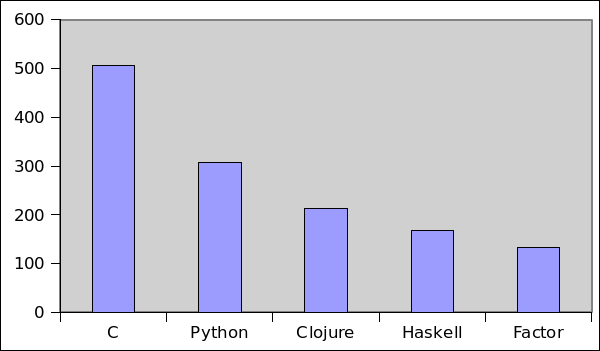
\includegraphics[width=4in]{graphs/total-lines-of-code.png}
    \caption{Total Lines of Code \label{fig:totallines}}
\end{figure}

Some languages pack more onto one line of source code than others.  In addition
to total lines, I calculated the number of tokens of each program, where a token
is any whitespace-separated string of characters (See
Table~\ref{tab:programcomparison} and Figure~\ref{fig:totaltokens}).  This gives
a measure of the program's ``density,'' that is, how much syntax is required to
express the total program.

\begin{figure}[h]
    \centering
    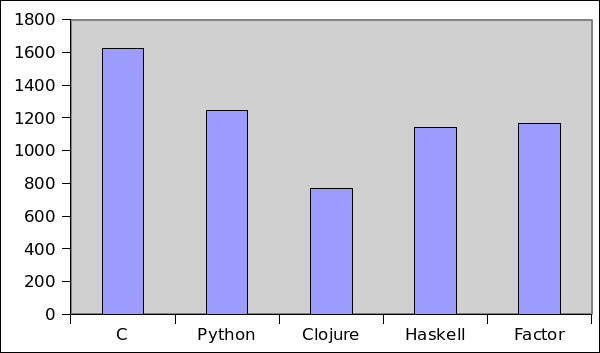
\includegraphics[width=4in]{graphs/total-tokens.png}
    \caption{Total Tokens \label{fig:totaltokens}}
\end{figure}

I was surprised to see that Clojure, though 3rd in line count, had the fewest
tokens.  Perhaps Clojure is the real winner in terms of expressiveness.

Average tokens per line, seen in Figure~\ref{fig:averagetokens}, is very telling
as well.  Factor, though having the fewest lines, is by far the densest program.
It sacrifices readability in some cases for compactness of code.  Clojure
manages to be tied for first in token density and still have the fewest tokens
overall.

\begin{figure}[h]
    \centering
    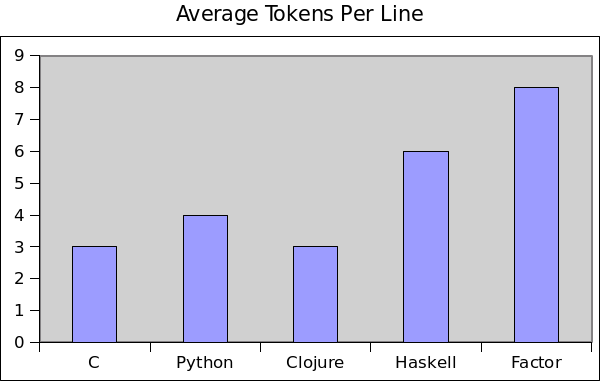
\includegraphics[width=4in]{graphs/average-tokens-per-line.png}
    \caption{Average Tokens Per Line \label{fig:averagetokens}}
\end{figure}

\section{Performance Comparisons}

To compare the performance of each language, I benchmarked each system playing
10,000 games of Farkle with four players on a 1.66 GHz netbook with 2 GB of RAM.
The operating system is Ubuntu 10.10.  The results are summarized in
table~\ref{tab:performance} and figure~\ref{fig:performance}.  Not surprisingly,
C performed best, taking around 13 seconds to complete.  Python was the slowest
at just over 10 minutes.

\begin{table}[h]
    \caption{Performance Summary \label{tab:performance}}
    \begin{tabular}{|p{1.2in}|p{0.3in}|p{0.5in}|p{0.5in}|p{0.5in}|p{0.5in}|}
        \hline
        {\bf Language} & {\bf C} & {\bf Python} & {\bf Clojure} & {\bf Haskell} & {\bf Factor} \\
        \hline
        {\bf Execution Time} & 0:13 & 10:10 & 3:50 & 3:15 & 5:30 \\
        \hline
    \end{tabular}
\end{table}

I was surprised by the performance of the other three languages.  Clojure claims
to be as fast or faster than Java, its host language, and Haskell claims to be
comparable in speed to C.  Factor compiles to machine code.  While each language
outperforms Python by quite a lot, none of them even approach C's speed.  Either
I am not writing idiomatic code (which is a very real possibility), or the
languages are not as fast as they claim.  Of course, all of the benchmarks I've
seen have been for toy problems, and the Farkle game is more of an actual
application.  The C code also doesn't do nearly as much as the rest of the
implementations.  The others are creating objects and allocating memory, but the
C code allocates memory once at the beginning and frees it at the end.

\begin{figure}[h]
    \centering
    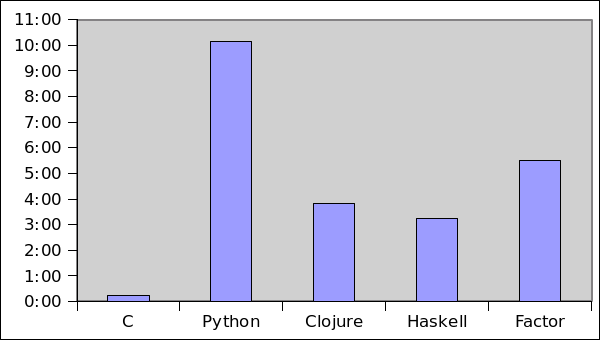
\includegraphics[width=4in]{graphs/performance-comparison.png}
    \caption{Execution Time for 10,000 4-Player Farkle Games \label{fig:performance}}
\end{figure}

Note that these times are for long runs of the programs.  On my netbook C,
Python, and Haskell start quickly, but Clojure takes a full 10
seconds to start, mostly due to it having to starting a new JVM instance.  Factor
takes about five seconds to reload code into its execution environment.

\section{Conclusions}
This project supports the idea that functional languages are more powerful than
procedural and object-oriented languages in terms of number of lines and tokens
required to express the same ideas.  However, some of the functional languages
may be suffering from idealism.

Haskell's quarantining of side effects enforces good programming practice, but
in the real world sometimes side effects make code simpler.  I have seen this
in the Farkle implementation in the generating of random numbers.  The Haskell
code required special constructs, but the Clojure code could just create random
numbers as needed anywhere in the code.

Another very helpful thing for a language is a strong community.  The more a
language is used, the more resources there will be for learning and the more
useful libraries that will be available.  Factor has many powerful features, but
it currently has a very small community.  There are almost no questions about it on
Stack Overflow, there are no books on Factor, and there is limited
documentation.  In contrast, the C and Python communities are vast.  The Haskell
and Clojure communities are small but increasing in size.

Python has always had as one of its big selling points that it is ``Batteries
Included:'' it comes with many useful libraries.  As the first or second
language on the TIOBE Index, C has libraries for anything due to its popularity
and age.  Haskell is coming closer to having the status of ``Batteries
Included'' as its community members continuously add to Hackage, the Haskell
library repository.  Clojure, already running on the JVM, made interfacing with
Java libraries seamless, allowing access to the huge amount of available Java
libraries.  Though Clojure is very young, Java interop gives it a running
start.

The purely functional programs are much easier to test than those with side
effects.  I am confident in the reliability of the Clojure and Haskell code that
I wrote.  This experience encourages me to write in a style that uses as few
side effects as possible --- even in procedural and object-oriented languages.  

With concurrency being as easy as it is in Clojure, I am reluctant to try to
implement a concurrent program in a language like Python.  Because Clojure can
automatically parallelize programs, it is an obvious choice for parallel
development.

I have learned a lot about different programming languages by doing this
project.  It is an exercise that I would recommend to any serious computer
scientist.  The more languages that I am exposed to, the more concepts that I
see being repeated and the more new concepts I learn.  This allows me to
approach problems in novel ways more often than if I only knew one language.

I have come to see that learning a new language in a paradigm I already know is
easy.  Once you know C++ you can then learn Java and C and PHP easily.  But it
is difficult to learn a language in a paradigm with which you do not have
experience.  \textsc{Lisp}-style languages and Haskell have taken me the most
time to learn of any other language simply because of the number of new features
and their new ways to do common tasks.  Some of these concepts, like Haskell's
monads and \textsc{Lisp's} macros simply take time to absorb.  I spent 10 weeks
on Haskell and I still don't understand everything.

Therefore, if I was going to choose a language for my next project, it would
probably be Clojure.  Of the languages I surveyed, it has the highest gain in
expressive power for the least amount of new concepts to learn.  I was very
impressed by Clojure's low total token count.  It is concise, but not so concise
that it is unreadable (like Factor).  It also is not so idealistic that it is
hard to use (like Haskell).

However, I have had experience with the functional paradigm.  If a team of
programmers are going to start a new project and they don't know the functional
paradigm, I would be reluctant to recommend Clojure.  Because learning a new
paradigm is hard, I would recommend using the most powerful language in the
paradigms known by the team.  For this, I would recommend Python.  It is still
procedural and object-oriented, but it is much more expressive than C, and
makes many common mistakes harder to do, e.g., off-by-one errors in loops.

The results of this investigation are summarized in table~\ref{tab:finalsummary}. 

\begin{table}[h]
    \caption{Summary of Language Features \label{tab:finalsummary}}
    \begin{tabular}{|p{0.7in}|p{0.7in}|p{0.7in}|p{0.7in}|p{0.7in}|p{0.7in}|}
        \hline
        {\bf Aspect} & {\bf C} & {\bf Python} & {\bf Clojure} & {\bf Haskell} & {\bf Factor} \\
        \hline
        {\bf Total~Lines of~Code} & 506 & 308 & 213 & 169 & 133 \\
        \hline
        {\bf Total Tokens} & 1627 & 1243 & 771 & 1142 & 1164 \\
        \hline
        {\bf Average Line Length} & 31 & 40 & 36 & 47 & 44 \\
        \hline
        {\bf Average Tokens Per Line} & 3 & 4 & 3 & 6 & 8 \\
        \hline
        {\bf 10,000 Game Execution Time} & 0:13 & 10:10 & 3:50 & 3:15 & 5:30 \\
        \hline
        {\bf Ease~of Learning} & Easy & Easy & Moderate & Difficult & Difficult \\
        \hline
        {\bf Purity} & Impure & Impure & Encourages Pure & Pure & Encourages Pure \\
        \hline
        {\bf Supported Paradigms} & Procedural & Procedural, Object-Oriented, Functional & Functional & Functional & Stack-based, Object-Oriented \\
        \hline
        {\bf Evaluation Strategy} & Eager & Eager & Lazy & Lazy & Eager \\
        \hline
        {\bf Execution Method} & Compiled & Interpreted & Byte-code Compiled & Compiled & Compiled \\
        \hline
    \end{tabular}
\end{table}

\section{Plans for Future Work}

I would like to see programs completed in Java, Erlang, and J.  I would also be
interested in seeing implementations in Scala, F\#, OCaml, Lua, and Groovy.
The more languages in the comparison, the more useful and informative it will
be.

One of the greatest flaws of my project is the fact that I was the only one
writing programs for comparison.  As such, my sample size is one.  I would love
to enlist the skills of prominent community members in each of
these languages and ask them to write the Farkle program.  Because I was just
learning some of these languages, my implementation may be much slower and
longer than what a master would produce.  I know that I did not make use of all
the advanced features of every language.  It would also be better if there were
more than one of each program.  Prechelt compiled many programs from various
programmers.  It would be an improvement to do the same for the Farkle
game.

It might be interesting for me to come back to this project in a few years
after I have matured as a programmer.  I have been trying to learn the
functional paradigm for several years now, and while I am getting better, I am
nowhere near fluent.  As I said above, learning a new language is easy, but
learning a new paradigm is hard.

\bibliographystyle{plain}
\bibliography{languages2}

\appendix
\section{Farkle Rules}
\label{sec:farklerules}

Farkle requires six dice.  On each turn, the player rolls all six dice and
removes combinations that are worth points.  The following combinations are
worth points:

\begin{itemize}
\item One 5 - 50 points
\item One 1 - 100 points
\item Three 1s - 300 points
\item Three 2s - 200 points
\item Three 3s - 300 points
\item Three 4s - 400 points
\item Three 5s - 500 points
\item Three 6s - 600 points
\item Four of a kind - 1000 points
\item 1-6 Straight   - 1500 points
\item Three pairs    - 1500 points
\item Five of a kind - 2000 points
\item Two triples    - 2500 points
\item Six of a kind  - 3000 points
\end{itemize}

To score, the combination must be removed all on the same turn.  As long as the
player can remove at least one die that scores, he or she can then continue to roll.
If the player cannot remove at least one die, they ``Farkle'' and lose all
points for that turn.  The strategy in the game comes from knowing when to stop
rolling and which dice to set aside.

\section{Source Code Listings}
The Farkle programs for each language, as well as the notes I took while learning them, can be found online in my Github repository~\cite{mygithub}.

\subsection{C Code}

\lstset{language=C,numbers=left,showspaces=false,showstringspaces=false,basicstyle=\footnotesize,numberstyle=\footnotesize}

\begin{lstlisting}
#include <stdio.h>
#include <stdlib.h>
#include <time.h>
#include <assert.h>

#define HUMAN_PLAYER 0
#define GREEDY_AI_PLAYER 1

#define E -1 //for empty

typedef struct {
    int type;
    int turn_score;
    int id;
    int threshold;
    int win_count;
} player;

player* create_player(int type, int id, int threshold);
void take_turn(player* p);
void query_human_set_aside(player* p, int* remaining,
                           int* set_aside, int* proposed_set_aside);
int query_human_stop(player* p, int* remaining, int* set_aside);

void query_greedy_player_set_aside(player* p, int* remaining,
                                   int* set_aside, int* proposed_set_aside);
int query_greedy_player_stop(player* p, int* remaining, int* set_aside);

int have_farkle(int* dice);
void roll_dice(int* dice);
int score_dice(int* dice);
void drop_n_dice(int* dice, int count);
void copy_dice(int* dice, int* copy);
int compare_dice_freqs(const void *a, const void *b);
void sort_by_frequency(int* dice);
int dice_contains(int* container, int* containee);
int remove_die(int* dice, int die);
int num_active_dice(int* dice);
void print_dice(char* msg, int* dice);

void run_tests();

int num_players = 4;
int cur_player = 0;
int total_scores[4] = {0, 0, 0, 0};
int die_counts[7] = {E, 0, 0, 0, 0, 0, 0};
int have_leftovers = 0;

int main()
{
    srand(time(0));
    player* players[4];
    int i, c;

    for (i=0; i<10000; i++){

        players[0] = create_player(GREEDY_AI_PLAYER, 0, 300);
        players[1] = create_player(GREEDY_AI_PLAYER, 1, 500);
        players[2] = create_player(GREEDY_AI_PLAYER, 2, 800);
        players[3] = create_player(GREEDY_AI_PLAYER, 3, 1000);

        for (c=0; c<num_players; c++){
            total_scores[c] = 0;
        }
        while(1){
            take_turn(players[cur_player]);
            if(total_scores[players[cur_player]->id] >= 10000){
                break;
            }
            cur_player += 1;
            if(cur_player == num_players){
                cur_player = 0;
            }
        }
        if (i%1000==0) printf("Done with game %d\n", i);
        players[cur_player]->win_count++;

        for(c=0; c<num_players; c++){
            free(players[c]);
        }

    }

    for(c=0; c<num_players; c++){
        printf("Player %d had %d wins.\n", players[c]->id, players[c]->win_count);
    }

    return 0;
}


void take_turn(player* p)
{
    int i,c;
    int stop;
    p->turn_score = 0;
    int remaining[6] = {0,0,0,0,0,0};
    int set_aside[6] = {E,E,E,E,E,E};
    int proposed_set_aside[6] = {E,E,E,E,E,E};
    for(i=0; i<6; i++){
        remaining[i] = 0;
        set_aside[i] = E;
    }
    while(1){
        roll_dice(remaining);

        if(have_farkle(remaining)){
            print_dice("You got a farkle!\nDice:", remaining);
            return;
        }
        switch (p->type) {
            case HUMAN_PLAYER:
                query_human_set_aside(p, remaining,
                                      set_aside, proposed_set_aside);
                break;
            case GREEDY_AI_PLAYER:
                query_greedy_player_set_aside(p, remaining,
                                              set_aside, proposed_set_aside);
                break;
        }

        p->turn_score += score_dice(proposed_set_aside);

        /* copy the user's choice into the set aside */
        int start = num_active_dice(set_aside);
        int end = start + num_active_dice(proposed_set_aside);
        for (i=start, c=0; i<end; i++, c++){
            set_aside[i] = proposed_set_aside[c];
        }
        /* and remove the user's choice from remaining */
        for (i=0; i<num_active_dice(proposed_set_aside); i++){
            remove_die(remaining, proposed_set_aside[i]);
        }

        /* if they set aside all dice, activate them all again */
        if(num_active_dice(remaining) == 0){
            for (i=0; i<6; i++){
                remaining[i] = 0;
            }
        }

        switch (p->type) {
            case HUMAN_PLAYER:
                stop = query_human_stop(p, remaining, set_aside);
                break;
            case GREEDY_AI_PLAYER:
                stop = query_greedy_player_stop(p, remaining, set_aside);
                break;
        }
        if (stop){
            total_scores[p->id] += p->turn_score;
            return;
        }
    }
}

int have_farkle(int* dice)
{
    return score_dice(dice) == 0;
}

void query_human_set_aside(player* p, int* remaining,
                           int* set_aside, int* proposed_set_aside){
    int i;
    char choice;
retry:

    for (i=0; i<6; i++) proposed_set_aside[i] = E;
    
    printf("Scores:\n");
    for(i=0; i<num_players; i++){
        printf("Player %d: %d\n", i, total_scores[i]);
    }

    printf("Turn score: %d\n", p->turn_score);

    print_dice("\nSet Aside: ", set_aside);

    print_dice("\nYou roll the dice: ", remaining);

    /* read in the set aside from the keyboard, retrying if it is invalid */
    for (i=0; i<6; i++) proposed_set_aside[i] = E;

    for (i=0; i<num_active_dice(remaining); i++){
        choice = getc(stdin);
        if(!(choice >= 49 && choice <= 54)){
            printf("That set aside is not valid! not real number\n");
            goto retry;
        }
        proposed_set_aside[i] = choice-48;
        choice = getc(stdin); /* eat the space */
        if(choice == '\n'){
            break;
        }
        if(choice != ' ') {
            printf("That set aside is not valid! not a space\n");
            printf("%d", choice);
            goto retry;
        }
    }
    if(num_active_dice(proposed_set_aside) == 0 ||
        num_active_dice(proposed_set_aside) > num_active_dice(remaining)){
        printf("That set aside is not valid! too many dice or zero\n");
        goto retry;
    }

    if(!dice_contains(remaining, proposed_set_aside)){
        printf("That set aside is not valid! dice not in set aside\n");
        goto retry;
    }

    int score = score_dice(proposed_set_aside);
    if(have_leftovers || score == 0){
        printf("That set aside is not valid! has leftovers or score is 0\n");
        goto retry;
    }
}

int query_human_stop(player* p, int* remaining, int* set_aside)
{
    char choice;
    printf("You have %d points.  Hit enter to continue rolling,
            or type 's' to end your turn.\n", p->turn_score);

    choice = getc(stdin);
    if (choice == '\n'){
        return 0;
    } else {
        while ( (choice = getc(stdin)) != '\n');
        return 1;
    }
}

void query_greedy_player_set_aside(player* p, int* remaining,
                                   int* set_aside, int* proposed_set_aside)
{
    int i, c;
    print_dice("\nAI player rolled:", remaining);

    for (c=0; c<6; c++){
        proposed_set_aside[c] = E;
    }

    if (num_active_dice(remaining) == 6 && score_dice(remaining) > 1000){
        copy_dice(remaining, proposed_set_aside);
    }
    sort_by_frequency(remaining);
    c = 0;
    for(i=0; i<6; i++){
        if (remaining[i] == 1 || remaining[i] == 5 ||
            die_counts[remaining[i]] >= 3){
            proposed_set_aside[c] = remaining[i];
            c++;
        }
    }
    
}

int query_greedy_player_stop(player* p, int* remaining, int* set_aside)
{
    return (p->turn_score >= p->threshold);
}


/* sets the global flag have_leftovers if there are unused dice */
int score_dice(int* dice)
{
    int score = 0;
    int i;

    int dice_copy[6];
    for (i=0; i<6; i++){
        dice_copy[i] = dice[i];
    }

    sort_by_frequency(dice_copy);    

    if (num_active_dice(dice_copy) == 6){
        /* six of a kind */
        if(dice_copy[0] == dice_copy[1] && dice_copy[0] == dice_copy[2] &&
           dice_copy[0] == dice_copy[3] && dice_copy[0] == dice_copy[4] &&
           dice_copy[0] == dice_copy[5]){
            drop_n_dice(dice_copy, 6);
            score += 3000;
        }

        /* two sets of three */
        if(dice_copy[0] != E && dice_copy[0] == dice_copy[1] &&
           dice_copy[0] == dice_copy[2] && dice_copy[3] == dice_copy[4] &&
           dice_copy[3] == dice_copy[5]){
            drop_n_dice(dice_copy, 6);
            score += 2500;
        }

        /* a set of four and a set of two */
        if(dice_copy[0] != E && dice_copy[0] == dice_copy[1] &&
           dice_copy[0] == dice_copy[2] && dice_copy[0] == dice_copy[3] &&
           dice_copy[4] == dice_copy[5]){
            drop_n_dice(dice_copy, 6);
            score += 1500;
        }

        /* three sets of two */
        if(dice_copy[0] != E && dice_copy[0] == dice_copy[1] &&
           dice_copy[2] == dice_copy[3] && dice_copy[4] == dice_copy[5]){
           drop_n_dice(dice_copy, 6);
            score += 1500;
        }

        /* straight */
        if(dice_copy[0] != E && dice_copy[0] == 1 && dice_copy[3] == 4 &&
           dice_copy[1] == 2 && dice_copy[4] == 5 &&
           dice_copy[2] == 3 && dice_copy[5] == 6){
            drop_n_dice(dice_copy, 6);
            score += 1500;
        }
    }

    if (num_active_dice(dice_copy) >= 5){
        /* five of a kind */
        if(dice_copy[0] == dice_copy[1] && dice_copy[0] == dice_copy[2] &&
             dice_copy[0] == dice_copy[3] && dice_copy[0] == dice_copy[4]){
            drop_n_dice(dice_copy, 5);
            score += 2000;
        }
    }

    if (num_active_dice(dice_copy) >= 4){
        /* four of a kind */
        if(dice_copy[0] == dice_copy[1] && dice_copy[0] == dice_copy[2] &&
           dice_copy[0] == dice_copy[3]){
            drop_n_dice(dice_copy, 4);
            score += 1000;
        }
    }

    if (num_active_dice(dice_copy) >= 3){
        /* three of a kind */
        if(dice_copy[0] == dice_copy[1] && dice_copy[0] == dice_copy[2]){
            if(dice_copy[0] == 1)
                score += 300;
            else
                score += dice_copy[0] * 100;
            drop_n_dice(dice_copy, 3);
        }
    }

    /* ones and fives */
    for (i=0; i<6; i++){
        if (dice_copy[i] == 1){
            dice_copy[i] = E;
            score += 100;
        }
        if (dice_copy[i] == 5){
            dice_copy[i] = E;
            score += 50;
        }
    }

    have_leftovers = 0;
    for (i=0; i<6; i++){
        if (dice_copy[i] != E){
            have_leftovers = 1;
        }
    }

    return score;
}

void drop_n_dice(int* dice, int count)
{
    int i;
    for (i=0; i<count; i++){
        remove_die(dice, dice[0]);
    }
}

void copy_dice(int* dice, int* copy)
{
    int i;
    for (i=0; i<6; i++){
        copy[i] = dice[i];
    }
}

int compare_dice_freqs(const void *a, const void *b)
{
    int die1 = *(const int *)a;
    int die2 = *(const int *)b;
    /* if we hit an E, the other is larger, if there is a tie,
     * sort by dot number, otherwise sort of die count */
    if(die1 == E) return 1;
    else if(die2 == E) return E;
    else if(die_counts[die1] == die_counts[die2]) return die2 - die1;
    else return die_counts[die2] - die_counts[die1];
}


void sort_by_frequency(int* dice)
{
    int i;
    /* find the counts of each die, referencing a global so
     * we can use them in the comparison function */
    for (i=1; i<=6; i++){
        die_counts[i] = 0;
    }
    for (i=0; i<6; i++){
        if(dice[i] != E)
            die_counts[dice[i]]++;
    }

    qsort(dice, 6, sizeof(int), compare_dice_freqs);
}



int dice_contains(int* container, int* containee)
{
    int container_copy[6];
    int containee_copy[6];
    int i;
    int die;
    for (i=0; i<6; i++){
        container_copy[i] = container[i];
        containee_copy[i] = containee[i];
    }

    while (num_active_dice(containee_copy) > 0) {
        die = containee_copy[0];
        remove_die(containee_copy, die);
        if(!remove_die(container_copy, die)){
            return 0;
        }
    }
    return 1;
}

/* returns true if it removed a die, otherwise false */
int remove_die(int* dice, int die)
{
    int i;
    for (i=0; i<6; i++){
        if(dice[i] == die){ 
            for (; i<5; i++){
                dice[i] = dice[i+1];
            }
            dice[5] = E;
            return 1;
        }
    }
    return 0;
}

int num_active_dice(int* dice)
{
    int i;
    for (i=0; i<6; i++){
        if(dice[i] == E){
            return i;
        }
    }
    return 6;
}

void print_dice(char* msg, int* dice)
{
    printf("%s", msg);
    int i;
    for(i=0; i<6; i++){
        if(dice[i] != E){ /* don't print out the die if it is inactive */
            printf("%d ", dice[i]);
        }
    }
    printf("\n");
    
}

void roll_dice(int* dice)
{
    int i;
    for(i=0; i<6; i++){
        if(dice[i] != E){
            dice[i] = rand() % 6 + 1;
        }
    }
}

player* create_player(int type, int id, int threshold)
{
    player *p = (player*) malloc(sizeof(player));

    p->type = type;
    p->turn_score = 0;
    p->id = id;
    p->threshold = threshold;

    return p;
}
\end{lstlisting}

\subsection{Python Code}

\lstset{language=Python,numbers=left,showspaces=false,showstringspaces=false,basicstyle=\footnotesize,numberstyle=\footnotesize}
\begin{lstlisting}
import random

class GreedyAIPlayer(object):

    def __init__(self, stop_threshold):
        self.stop_threshold = stop_threshold

    def query_set_aside(self, remaining, set_aside, turn_score, total_scores):

        dice_score = remaining.get_score()
        if remaining.count() == 6 and dice_score >= 1500 and dice_score != 2000:
            return remaining.get_values()

        result = []
        counts = remaining.get_counts()
        for die, count in counts.iteritems():
            if die == 1 or die == 5 or count >= 3:
                result.extend([die] * count)
        return result

    def query_stop(self, remaining, set_aside, turn_score, total_scores):
        if turn_score >= self.stop_threshold:
            return True
        else:
            return False

    def warn_invalid_set_aside(self):
        pass # the AI should never set aside invalidly

    def warn_farkle(self, roll):
        pass

class HumanPlayer(object):

    def query_set_aside(self, remaining, set_aside, turn_score, total_scores):
        print "\n\nScores:\n"
        for i, score in enumerate(total_scores):
            print "Player {0}: {1}".format(i, score)

        print "Turn score: ", turn_score

        print "\nSet Aside:"
        print set_aside.get_values_as_string()

        print "\nYou roll the dice:"
        print remaining.get_values_as_string()

        choices = raw_input("\nIndicate the dice you want to set aside by
                              entering their numbers separated by spaces.\n")

        try:
            return [int(choice) for choice in choices.split()]
        except ValueError:
            return ''

    def query_stop(self, remaining, set_aside, turn_score, total_scores):
        choice = raw_input("You have {0} points.  Hit enter to continue rolling,
                            or type 'stop' to end your turn.\n".format(turn_score))
        if choice == '':
            return False
        else:
            return True

    def warn_invalid_set_aside(self):
        print "That set aside is invalid!"

    def warn_farkle(self, roll):
        print "You got a farkle!"
        print "Dice: " + roll.get_values_as_string()

class InvalidSetAsideException(Exception):
    pass

class GotFarkleException(Exception):
    pass

class BadDieException(Exception):
    pass

class DiceFactory(object):

    @staticmethod
    def rolled_dice(count):
        dice = Dice()
        dice.values = [random.randint(1, 6) for die in range(count)]
        return dice

    @staticmethod
    def set_as(values):
        for die in values:
            if not (1 <= die <= 6):
                raise BadDieException()
        dice = Dice()
        dice.values = list(values)
        return dice


class Dice(object):

    def __init__(self):
        self.counts = None

    def count(self):
        return len(self.values)

    def get_most_valuable_single_die(self):
        counts = self.get_counts()
        if counts[1] > 0:
            return (1,)
        elif counts[5] > 0:
            return (5,)
        else:
            return None
            
    def get_most_valuable_set_aside(self):
        counts = self.get_counts()

        # 4 of a kind with a pair and 3 pairs
        # are the only scoring combinations with a pair of dice
        if counts.values().count(4) and counts.values().count(2):
            return self.get_values()
        if counts.values().count(2) == 3:
            return self.get_values()
        
        result = []
        for die, count in counts.iteritems():
            if count >= 3 or die == 1 or die == 5:
                result.extend([die]*count)
        return tuple(result)


    def all_dice_score(self):
        counts = self.get_counts()
        if (((counts[2] >= 3 or counts[2] ==0) and
             (counts[3] >= 3 or counts[3] ==0) and
             (counts[4] >= 3 or counts[4] ==0) and
             (counts[6] >= 3 or counts[6] ==0))
            or
            (counts.values().count(4) and
             counts.values().count(2))):
            return True
        else:
            return False

    def contains_three_of_a_kind_and_two_others(self, i):
        counts = self.get_counts()

        if i == 1 and counts[1] == 3 and counts[5] == 2: return True
        if i == 5 and counts[5] == 3 and counts[1] == 2: return True

        if ((i == 2 and counts[2] == 3 and counts[3] < 3
                    and counts[4] < 3 and counts[6] < 3) or
            (i == 3 and counts[2] < 3 and counts[3] == 3
                    and counts[4] < 3 and counts[6] < 3) or
            (i == 4 and counts[2] < 3 and counts[3] < 3
                    and counts[4] == 3 and counts[6] < 3) or
            (i == 6 and counts[2] < 3 and counts[3] < 3
                    and counts[4] < 3 and counts[6] == 3)):

            if (counts[1] == 2 and counts[5] == 0) or
               (counts[5] == 2 and counts[1] == 0) or
               (counts[1] == 1 and counts[5] == 1):
                return True
            else:
                return False
        else:
            return False

    def contains_three_of_a_kind_and_one_other(self, i):
        counts = self.get_counts()

        if i == 1 and counts[1] == 3 and counts[5] == 1: return True
        if i == 5 and counts[5] == 3 and counts[1] == 1: return True

        if ((i == 2 and counts[2] == 3 and counts[3] < 3
                    and counts[4] < 3 and counts[6] < 3) or
            (i == 3 and counts[2] < 3 and counts[3] == 3
                    and counts[4] < 3 and counts[6] < 3) or
            (i == 4 and counts[2] < 3 and counts[3] < 3
                    and counts[4] == 3 and counts[6] < 3) or
            (i == 6 and counts[2] < 3 and counts[3] < 3
                    and counts[4] < 3 and counts[6] == 3)):

            if (counts[1] == 1 and counts[5] == 0) or
               (counts[5] == 1 and counts[1] == 0):
                return True
            else:
                return False
        else:
            return False

    def contains_n_or_more_of_a_kind(self, n):
        return any(map(lambda (die,count): count >= n,
                   self.get_counts().iteritems()))

    def contains_only_three_of_a_kind(self):
        die_counts = self.get_counts()
        if ((die_counts[1] == 0 or die_counts[1] == 3) and
            (die_counts[5] == 0 or die_counts[5] == 3) and 
            (any(map(lambda (die,count): count==3, die_counts.iteritems())))):
            return True
        else:
            return False

    def contains_one_scoring_die(self):
        if self.contains_n_or_more_of_a_kind(3):
            return False

        die_counts = self.get_counts()
        if die_counts[1] == 1 and die_counts[5] == 0 or
           die_counts[1] == 0 and die_counts[5] == 1:
            return True
        else:
            return False

    def get_counts(self):
        if self.counts == None:
            die_counts = {1:0, 2:0, 3:0, 4:0, 5:0, 6:0}
            for die in self.values:
                die_counts[die] += 1
            self.counts = die_counts
        return self.counts


    def get_values(self):
        return tuple(self.values)

    def have_one_of_each(self):
        counts = self.get_counts()
        return all([counts[die] > 0 for die in range(1, 7)])

    def get_values_as_string(self):
        return ' '.join([str(die) for die in self.get_values()])

    def is_valid_set_aside(self, remaining):
        if not remaining.contains_values(self):
            return False
        if self.get_score(zero_for_extra=True) == 0:
            return False
        return True

    def contains_values(self, dice):
        proposed_dice = list(dice.get_values())
        for die in self.get_values():
            if die in proposed_dice:
                proposed_dice.remove(die)
        return len(proposed_dice) == 0

    def is_farkle(self):
        return self.get_score() == 0

    def find_n_of_a_kind(self, n):
        matches = []
        die_counts = self.get_counts()
        for i in range(1,7):
            if die_counts[i] >= n:
                matches.append(i)
        return tuple(matches)

    def add(self, new_dice):
        self.values.extend(new_dice.get_values())

    def remove(self, dice):
        for die_value in dice.get_values():
            self.values.remove(die_value)

    def get_score(self, zero_for_extra=False, return_extra=False):
        score = 0
        die_counts = self.get_counts()

        # four with a pair, two triplets, three pairs, strait,
        # and 6 of a kind can all just return their point value
        # because they use all the dice
        if die_counts.values().count(4) and die_counts.values().count(2):
            return 1500
        if die_counts.values().count(3) == 2:
            return 2500
        if die_counts.values().count(2) == 3:
            return 1500
        if self.have_one_of_each():
            return 1500
        if die_counts.values().count(6):
            return 3000

        #3, 4, and 5 of a kind
        if die_counts.values().count(5):
            score += 2000
            if die_counts[1] == 1: score += 100
            if die_counts[5] == 1: score += 50
            if zero_for_extra and (die_counts[2] == 1 or
                                   die_counts[3] == 1 or
                                   die_counts[4] == 1 or
                                   die_counts[6] == 1):
                score = 0
            return score

        if die_counts.values().count(4):
            score += 1000
            if die_counts[1] <= 2: score += 100 * die_counts[1]
            if die_counts[5] <= 2: score += 50 * die_counts[5]
            if zero_for_extra and (1 <= die_counts[2] <= 2 or
                                   1 <= die_counts[3] <= 2 or
                                   1 <= die_counts[4] <= 2 or
                                   1 <= die_counts[6] <= 2):
                score = 0
            return score

        for die in range(1,7):
            if die_counts[die] == 3:
                if die == 1:
                    score += 300
                else:
                    score += die * 100
        if 1 <= die_counts[1] <= 2: score += 100 * die_counts[1]
        if 1 <= die_counts[5] <= 2: score += 50 * die_counts[5]
        if zero_for_extra and (1 <= die_counts[2] <= 2 or
                               1 <= die_counts[3] <= 2 or
                               1 <= die_counts[4] <= 2 or
                               1 <= die_counts[6] <= 2):
            score = 0
        return score

class NotEnoughPlayersException(Exception):
    pass

class Farkle(object):

    def __init__(self):
        self.players = []
        self.scores = []
        self.turn_index = 0

    def add_player(self, player):
        self.players.append(player)
        self.scores.append(0)

    def play(self):
        if len(self.players) == 0: raise NotEnoughPlayersException()

        while True:
            score = self.take_turn()
            self.scores[self.turn_index] += score

            if self.scores[self.turn_index] > 10000: break
            self.turn_index += 1
            if self.turn_index > len(self.players) - 1: self.turn_index = 0

        return self.turn_index

    def take_turn(self):
        player = self.players[self.turn_index]
        turn_score = 0
        set_aside = DiceFactory.set_as(())
        #junk value to initialize the number of dice
        remaining = DiceFactory.set_as((1,1,1,1,1,1))

        while True:
            remaining = DiceFactory.rolled_dice(remaining.count())
            if remaining.is_farkle():
                player.warn_farkle(remaining)
                return 0

            while True:
                proposed_set_aside =
                    DiceFactory.set_as(player.query_set_aside(remaining,
                                                              set_aside,
                                                              turn_score,
                                                              tuple(self.scores)))

                if proposed_set_aside.is_valid_set_aside(remaining):
                    remaining.remove(proposed_set_aside)
                    set_aside.add(proposed_set_aside)
                    break
                else:
                    player.warn_invalid_set_aside()

            turn_score += proposed_set_aside.get_score()
            if player.query_stop(remaining, set_aside, turn_score, tuple(self.scores)):
                return turn_score
            if remaining.count() == 0:
                remaining = DiceFactory.set_as((1,1,1,1,1,1))
                set_aside = DiceFactory.set_as(())

def lists_are_same(lst1, lst2):
    for e1, e2 in zip(lst1, lst2):
        if e1 != e2:
            return False
    return True

def main():
    wins = [0, 0, 0, 0]
    for i in range(10000):
        if i % 100 == 0:
            print "Game", i
        farkle = Farkle()
        farkle.add_player(GreedyAIPlayer(300))
        farkle.add_player(GreedyAIPlayer(500))
        farkle.add_player(GreedyAIPlayer(800))
        farkle.add_player(GreedyAIPlayer(1000))
        winner = farkle.play()
        wins[winner] += 1
    for i, win in enumerate(wins):
        print "Player", i, "had", win, "wins."

if __name__ == "__main__":
    main()
\end{lstlisting}

\subsection{Clojure Code}

\lstset{language=Lisp,numbers=left,showspaces=false,showstringspaces=false,basicstyle=\footnotesize,numberstyle=\footnotesize}
\begin{lstlisting}
(ns farkle.core
  (:use clojure.contrib.str-utils)
  (:use clojure.test clojure.set)
  (:gen-class)
  )

(defn third [x]
  (first (next (next x))))

(defn sort-by-frequency [lst]
  (let [counts (seq (frequencies lst))]
    (sort
     (fn [a b]
       (let [comp (compare (second b)
			   (second a))]
	 (if (= comp 0)
	   (compare (first a)
		    (first b))
	   comp)))
     counts)))

(defn value-of-extra-1s-and-5s [dice]
  (let [freqs (frequencies dice)]
    (+ (if (<= (freqs 1 0) 2)
         (* (freqs 1 0) 100)
         0)
       (if (<= (freqs 5 0) 2)
         (* (freqs 5 0) 50)
         0))))

(defn have-straight? [dice]
  (= (sort dice)
     (range 1 7)))

(defn roll-has-nonscoring-dice [dice]
  (let [die-map (frequencies dice)]
    (not
      (every? true? (map #(or (or (= (val %) 0)
                                  (<= 3 (val %) 6))
                              (= (key %) 1)
                              (= (key %) 5))
                         die-map)))))

(defn get-score
  ([dice] (get-score dice false))
  ([dice zero-for-extra]
   (if (= (count dice) 0)
     0
     (let [die-counts (sort-by-frequency dice)
           [fst-die fst-cnt] (first die-counts)
           [snd-die snd-cnt] (second die-counts)
           [trd-die trd-cnt] (third die-counts)
           single-dice-value (value-of-extra-1s-and-5s dice)]
       (cond
         (and (= fst-cnt 4) (= snd-cnt 2)) 1500
         (and (= fst-cnt 3) (= snd-cnt 3)) 2500
         (and (= fst-cnt 2) (= snd-cnt 2) (= trd-cnt 2)) 1500
         (have-straight? dice) 1500
         (= fst-cnt 6) 3000
         (and zero-for-extra (roll-has-nonscoring-dice dice)) 0
         (= fst-cnt 5) (+ single-dice-value 2000)
         (= fst-cnt 4) (+ single-dice-value 1000)
         (= fst-cnt 3) (+ single-dice-value
                          (if (= fst-die 1)
                            300
                            (* fst-die 100)))
         :else single-dice-value)))))

(defn contains-values [first-vals second-vals]
  (loop [container (sort first-vals)
         containee (sort second-vals)]
    (if (= (count containee) 0)
      true
      (if (= (count container) 0)
        false
        (if (= (first container)
               (first containee))
          (recur (rest container)
                 (rest containee))
          (recur (rest container)
                 containee))))))

(defn is-valid-set-aside [remaining new-set-aside]
  (and (contains-values remaining new-set-aside)
       (> (get-score new-set-aside true) 0)))

(defn is-farkle [dice]
  (= (get-score dice) 0))

(defn contains-one-scoring-die [dice]
  (let [freqs (frequencies dice)]
    (and (< (freqs 2) 3)
         (< (freqs 3) 3)
         (< (freqs 4) 3)
         (< (freqs 6) 3)
         (or (and (= (freqs 1) 1)
                  (= (freqs 5) 0))
             (and (= (freqs 1) 0)
                  (= (freqs 5) 1))))))

(defn contains-only-three-of-a-kind [dice]
  (let [freqs (frequencies dice)]
    (and (not (<= 1 (freqs 1) 2))
         (not (<= 1 (freqs 5) 2))
         (= (reduce + (map #(if (= (val %) 3) 1 0) freqs)) 1))))

(defprotocol FarklePlayer
  (get-name [this])
  (query-set-aside [this remaining set-aside turn-score total-scores])
  (query-stop [this remaining set-aside turn-score total-scores])
  (warn-invalid-set-aside [this])
  (warn-farkle [this roll]))

(deftype GreedyAIPlayer [name stop-threshold]
  FarklePlayer
  (get-name [this]
    name)
  (query-set-aside [this remaining set-aside turn-score total-scores]
    (let [dice-score (get-score remaining)]
      (if (and (= (count remaining) 6)
               (or (= dice-score 1500)
                   (= dice-score 2500)
                   (= dice-score 3000)))
        remaining
        (let [freqs (frequencies remaining)
              new-set-aside (filter #(or (>= (freqs %) 3)
                                         (= % 1)
                                         (= % 5))
                                    remaining)]
            new-set-aside))))

  (query-stop [this remaining set-aside turn-score total-scores]
    (> turn-score stop-threshold))
    
  (warn-invalid-set-aside [this]
                          )

  (warn-farkle [this roll]
               )
  )

(deftype HumanPlayer [name]
  FarklePlayer
  (get-name [this]
    name)
  (query-set-aside [this remaining set-aside turn-score total-scores]
    (println "\n\nScores:\n")
    (doseq [[i score] (map-indexed vector total-scores)]
      (println (format "Player %d: %d" i score)))
    (println "Turn score:" turn-score)
    
    (println "Set Aside:")
    (println set-aside)
    
    (println "You roll the dice:")
    (println remaining)
    (println "Indicate the dice you want to set aside
              by entering their numbers separated by spaces.")

    (let [choices (read-line)]
      (map #(Integer/parseInt %) (re-split #" " choices))))

  (query-stop [this remaining set-aside turn-score total-scores]
    (println
      (format
        "You have %d points.  Hit enter to continue rolling,
         or type 'stop' to end your turn."
        turn-score))
    (let [choice (read-line)]
      (if (= choice "")
        false
        true)))

  (warn-invalid-set-aside [this]
    (println "That set aside is invalid!"))

  (warn-farkle [this roll]
    (println "You got a farkle!")
    (println "Dice:" roll))
)

(defn roll-dice [num-to-roll]
  (for [die (range num-to-roll)]
    (inc (rand-int 6))))

(defn get-validated-set-aside [player remaining set-aside
                               turn-score total-scores]
  (loop [new-set-aside (query-set-aside player remaining set-aside
                                        turn-score total-scores)]
    (if (is-valid-set-aside remaining new-set-aside)
      new-set-aside
      (do
        (warn-invalid-set-aside player)
        (recur (query-set-aside player remaining set-aside
                                turn-score total-scores))))))

(defn take-turn [player total-scores]
  (loop [turn-score 0
         set-aside []
         remaining (roll-dice 6)]
    (if (is-farkle remaining)
      (do
        (warn-farkle player remaining)
        0)
      (let [new-set-aside (get-validated-set-aside player remaining set-aside
                                                   turn-score total-scores)
            new-turn-score (+ turn-score (get-score new-set-aside))]
        (if (query-stop player remaining set-aside
                        new-turn-score total-scores)
          new-turn-score
          (recur new-turn-score
                 (concat set-aside new-set-aside)
                 (roll-dice (let [die-count (- (count remaining)
                                               (count new-set-aside))]
                              (if (> die-count 0)
                                die-count
                                6)))))))))

(defn play-farkle [players]
  (if (= (count players) 0)
    (println "Not enough players!")
    (loop [rotation (cycle players)
	   scores (zipmap players (repeat 0))]
      (let [player (first rotation)
	    updated-score (+ (scores player)
                         (take-turn player (take (count players)
                                                 (vec
                                                   (map val scores)))))]
        (if (>= updated-score 10000)
          player
          (recur (rest rotation)
                 (assoc scores player updated-score)))))))

(defn -main [& args]
  (loop [times 10000]
    (let [winner (play-farkle [(GreedyAIPlayer. "Greedy Player 1" 300)
                               (GreedyAIPlayer. "Greedy Player 2" 500)
                               (GreedyAIPlayer. "Greedy Player 3" 800)
                               (GreedyAIPlayer. "Greedy Player 4" 1000)])]
      (do
        (if (= (mod times 1000) 0) (println times " games left."))
        (if (> times 0)
          (recur (- times 1))
          (println "Done"))))))
\end{lstlisting}

\subsection{Haskell Code}

\lstset{language=Haskell,numbers=left,showspaces=false,showstringspaces=false,basicstyle=\footnotesize,numberstyle=\footnotesize}
\begin{lstlisting}
{-# LANGUAGE TypeSynonymInstances #-}
module Main where

import Data.List
import Debug.Trace
import Data.Monoid
import Text.Printf
import System.Random

data Player = Player { name :: String
                     , score :: Int
                     , threshold :: Int
                     , kind :: PlayerType
                     } deriving (Show)

--maybe this should be in the state monad eh?
data TurnState = TurnState { remaining :: [Int]
                           , setAside :: [Int]
                           , turnScore :: Int }

data PlayerType = HumanPlayer | GreedyAIPlayer | GAPlayer deriving (Show)

main :: IO ()
main = do putStrLn "Purely functional Farkle in Haskell!"
          repeatFarkle 10000

repeatFarkle :: Int -> IO ()
repeatFarkle times = do
          let players = [Player {name = "AI Player 1", score = 0,
                                 threshold = 300, kind = GreedyAIPlayer}
                        ,Player {name = "AI Player 2", score = 0,
                                 threshold = 500, kind = GreedyAIPlayer}
                        ,Player {name = "AI Player 3", score = 0,
                                 threshold = 800, kind = GreedyAIPlayer}
                        ,Player {name = "AI Player 4", score = 0,
                                 threshold = 1000, kind = GreedyAIPlayer}
                        ]

          winner <- playFarkle players
          if times > 0
             then do
              if times `mod` 1000 == 0
                then putStrLn (show times ++ " games left.")
                else return ()
              repeatFarkle (times - 1)
             else return ()


playFarkle :: [Player] -> IO Player
playFarkle players@(curPlayer:otherPlayers) = do
    newCurPlayer <- takeTurn curPlayer (getScores players)
    if score newCurPlayer >= 10000
       then return newCurPlayer
       else do
           playFarkle $ otherPlayers ++ [newCurPlayer]

getScores :: [Player] -> [Int]
getScores players =
    map score players

--It would appear that the game structure, being very procedural in nature,
--does not benefit from a purely functional model
takeTurn :: Player -> [Int] -> IO Player
takeTurn player totalScores = do
    initialDice <- rollDice [0,0,0,0,0,0]
    turnLoop TurnState {remaining = initialDice, setAside = [], turnScore = 0} 
    where turnLoop turnState
            | isFarkle $ remaining turnState = do
                warnFarkle (kind player) (remaining turnState)
                return player
            | otherwise = do
                newSetAside <- querySetAside (kind player) turnState totalScores
                newRoll <- rollDice
                            (if length (setAside turnState) + length newSetAside == 6
                                then [0,0,0,0,0,0]
                                else removeElems newSetAside (remaining turnState))
                let newTurnState =
                        TurnState { remaining = newRoll
                                  , setAside = (if length newRoll == 6
                                                    then []
                                                    else setAside turnState ++
                                                         newSetAside)
                                  , turnScore = turnScore turnState +
                                                fst (findScore newSetAside) }
                choice <- queryStop (kind player) (threshold player)
                                    newTurnState totalScores
                if choice == True
                   then do return $ player { score = 
                                               score player + turnScore newTurnState }
                   else do turnLoop newTurnState

removeElems :: (Eq a) => [a] -> [a] -> [a]
removeElems [] lst = lst
removeElems (x:xs) lst = removeElems xs (delete x lst)

rollDice :: [Int] -> IO [Int]
rollDice dice = do
    newDice <- sequence $ replicate (length dice) $ getStdRandom $ randomR (1,6)
    return newDice

isFarkle :: [Int] -> Bool
isFarkle dice = fst (findScore dice) == 0

querySetAside :: PlayerType -> TurnState -> [Int] -> IO [Int]
querySetAside HumanPlayer turnState totalScores = do
    putStrLn "\n\nScores:\n"
    --uncurry: convert a two argument function to a
    --one argument function that operates on a pair
    mapM_ (uncurry $ printf "Player %d: %d\n") ((zip ([1..] :: [Int]) totalScores))

    putStrLn $ "Turn score: " ++ show (turnScore turnState)
    putStrLn "\nSet Aside:"
    putStrLn $ show $ setAside turnState

    putStrLn "\nYou roll the dice:"
    putStrLn $ show $ remaining turnState
    putStrLn "\nIndicate the dice you want to set aside by
              entering their numbers separated by spaces.\n"
    choice <- getLine
    let setAside = map read (words choice)
    if (length setAside > 0) &&
        containsValues setAside (remaining turnState) &&
        length (snd (findScore setAside)) == 0
       then return setAside
       else do
           putStrLn "That set aside is not valid!"
           querySetAside HumanPlayer turnState totalScores

querySetAside GreedyAIPlayer turnState totalScores = do
    if length (remaining turnState) == 6 && fst (findScore (remaining turnState)) > 1000
       then return $ remaining turnState
       else do
           let newSetAside = filter isScoringDie (remaining turnState)
           return newSetAside
    where isScoringDie die =
              die == 1 || die == 5 ||
              (length (filter (== die) (remaining turnState)) == 3)

containsValues :: (Eq a, Ord a) => [a] -> [a] -> Bool
containsValues firstVals secondVals =
    containsValues' (sort firstVals) (sort secondVals)
    where containsValues' [] _ = True
          containsValues' _ [] = False
          containsValues' (x:xs) (y:ys)
            | x == y = containsValues' xs ys
            | otherwise = containsValues' (x:xs) ys
    
queryStop :: PlayerType -> Int -> TurnState -> [Int] -> IO Bool
queryStop HumanPlayer threshold turnState totalScores = do
    putStrLn $ "You have " ++ (show $ turnScore turnState) ++
               ".  Hit enter to continue rolling, or type 'stop' to end your turn.\n"
    choice <- getLine
    if choice == "" then do return False else do return True

queryStop GreedyAIPlayer threshold turnState totalScores = do
    return $ turnScore turnState > threshold

warnFarkle :: PlayerType -> [Int] -> IO ()
warnFarkle HumanPlayer dice = do
    putStrLn $ "You got a farkle!\nDice: " ++ show dice

warnFarkle GreedyAIPlayer dice = do
    return ()

sortByFrequency :: (Ord a, Eq a) => [a] -> [a]
sortByFrequency lst = sortBy moreInList lst
    where moreInList x y = ((numInList y) `compare` (numInList x))
                                          `mappend` (x `compare` y)
          --use the Ord monoid to sort by different criteria;
          --if the first gives an EQ, the second applies
          numInList e = length $ filter (== e) lst

--not sure if I could use a monad here?
--Chaining score and remaining dice filtering functions
findScore :: [Int] -> (Int, [Int])
findScore dice =
    remove1s5s . (removeNOfAKind 3) . (removeNOfAKind 4) . (removeNOfAKind 5)
        . remove222 . remove33 . remove42 . removeStraight . (removeNOfAKind 6)
        $ (0, sortByFrequency dice) 

-- Expects the dice to be sorted by frequency
remove42 :: (Int, [Int]) -> (Int, [Int])
remove42 (score, dice)
    | length dice /= 6 = (score, dice)
    | all (== head first4) first4 && all (== head last2) last2 = (score + 1500, [])
    | otherwise = (score, dice)
    where (first4, last2) = splitAt 4 dice

remove33 :: (Int, [Int]) -> (Int, [Int])
remove33 (score, dice)
    | length dice /= 6 = (score, dice)
    | all (== head first3) first3 && all (== head last3) last3 = (score + 2500, [])
    | otherwise = (score, dice)
    where (first3, last3) = splitAt 3 dice

remove222 :: (Int, [Int]) -> (Int, [Int])
remove222 (score, dice)
    | length dice /= 6 = (score, dice)
    | all (== head first2) first2 && all (== head mid2) mid2 &&
      all (== head last2) last2 = (score + 2500, [])
    | otherwise = (score, dice)
    where (first2, rest) = splitAt 2 dice
          (mid2, last2) = splitAt 2 rest

remove1s5s :: (Int, [Int]) -> (Int, [Int])
remove1s5s (score, dice) =
    let (onesAndFives, rest) = partition (\x -> x == 1 || x == 5) dice
        valOf1s5s = sum $ map getScore onesAndFives
    in (score + valOf1s5s, rest)
    where getScore 1 = 100
          getScore 5 = 50

removeStraight :: (Int, [Int]) -> (Int, [Int])
removeStraight (score, dice)
    | sort dice == [1,2,3,4,5,6] = (score + 1500, [])
    | otherwise = (score, dice)

removeNOfAKind :: Int -> (Int, [Int]) -> (Int, [Int])
removeNOfAKind n (score, dice)
    | length dice < n = (score, dice)
    | all (== head dice) firstN = (score + scoreNOfAKind firstN, drop n dice)
    | otherwise = (score, dice)
    where firstN = take n dice
          scoreNOfAKind dice =
              case length dice of 
                   6 -> 3000
                   5 -> 2000
                   4 -> 1000
                   3 -> if head dice == 1 then 300 else (head dice) * 100
                   otherwise -> error "Should not try to take another n of a kind"
\end{lstlisting}

\subsection{Factor Code}

\lstset{language=C,numbers=left,showspaces=false,showstringspaces=false,basicstyle=\footnotesize,numberstyle=\footnotesize}
\begin{lstlisting}
USING: kernel random math sequences prettyprint io formatting
accessors fry locals math.order sorting splitting math.parser
combinators tools.continuations ;
IN: farkle

: rotate ( seq -- seq ) dup first suffix 0 swap remove-nth ;

: roll-dice ( x -- seq ) [ 6 random 1 + ] replicate ;

: count ( elt seq -- cnt ) swap '[ _ = ] filter length ;

:: sort-by-frequency ( arr -- seq )
    arr [ 2dup [ arr count ] bi@ >=<
            dup +eq+ = [ drop <=> ] [ 2nip ] if
        ] sort ;
    
: all-eq? ( seq -- ? ) dup first '[ _ = ] all? ;

: must-have ( seq score block count -- seq score )
    [ over ] 2dip rot length <= swap when ; inline
    

: (score-6) ( seq score -- seq score ) [ over all-eq?
    [ 3000 [ 6 tail ] 2dip ] [ 0 ] if + ] 6 must-have ;

: (score-42) ( seq score -- seq score ) [ over
    [ 4 head all-eq? ] [ 4 tail all-eq? ] bi and
    [ 1500 [ 6 tail ] 2dip ] [ 0 ] if + ] 6 must-have ;

: (score-33) ( seq score -- seq score ) [ over
    [ 3 head all-eq? ] [ 3 tail all-eq? ] bi and
    [ 2500 [ 6 tail ] 2dip ] [ 0 ] if + ] 6 must-have ;

: (score-222) ( seq score -- seq score ) [ over
    [ 2 head all-eq? ] [ 2 4 rot subseq all-eq? ]
    [ 4 tail all-eq? ] tri and and
    [ 1500 [ 6 tail ] 2dip ] [ 0 ] if + ] 6 must-have ;

: (score-straight) ( seq score -- seq score ) [ over
    { 1 2 3 4 5 6 } =
    [ 1500 [ 6 tail ] 2dip ] [ 0 ] if + ] 6 must-have ;

: (score-5) ( seq score -- seq score ) [ over 5 head all-eq?
    [ 2000 [ 5 tail ] 2dip ] [ 0 ] if + ] 5 must-have ;

: (score-4) ( seq score -- seq score ) [ over 4 head all-eq?
    [ 1000 [ 4 tail ] 2dip ] [ 0 ] if + ] 4 must-have ;


: (3s-score) ( seq -- score ) first dup 1 =
    [ drop 300 ] [ 100 * ] if ;

: (score-3) ( seq score -- seq score ) [ over 3 head all-eq?
    [ over (3s-score) [ 3 tail ] 2dip ] [ 0 ] if + ] 3 must-have ;


: (score-1s5s) ( seq score -- seq score ) swap
    [ [ [ 1 = not ] [ 5 = not ] bi and ] filter ]
    [ [ 1 = ] filter length 100 * ] 
    [ [ 5 = ] filter length 50 * ] tri + swap [ + ] dip swap ;


: score-dice ( seq -- leftovers score )
    sort-by-frequency 0 (score-6) (score-42)
    (score-33) (score-222) (score-straight)
    (score-5) (score-4) (score-3) (score-1s5s) ;

: farkle? ( seq -- ? )
    score-dice 0 = nip ;


: string>array ( str -- arr ) " " split [ string>number ] map ;

: array>string ( arr -- str ) [ number>string ] map " " join ;

: (contains-values?) ( container containee -- ? )
    {
        { [ dup length 0 = ] [ 2drop t ] }
        { [ over length 0 = ] [ 2drop f ] }
        { [ 2dup [ first ] bi@ = ] 
            [ [ rest ] bi@ (contains-values?) ] }
        [ [ rest ] dip (contains-values?) ] 
    } cond ;

: contains-values? ( container containee -- ? ) 
    [ [ <=> ] sort ] bi@ (contains-values?) ;


TUPLE: turn-state remaining set-aside turn-score ;
: <turn-state> ( -- turn-state ) 6 roll-dice { } 0 turn-state boa ;

TUPLE: human-player name score win-count ;

: <human-player> ( name -- human-player ) 0 0 human-player boa ;

TUPLE: greedy-ai-player threshold name score win-count ;

: <greedy-ai-player> ( threshold name -- greedy-ai-player )
    0 0 greedy-ai-player boa ;

GENERIC: query-set-aside ( state player -- set-aside )
M: human-player query-set-aside ( state player -- set-aside )
    swap dup remaining>> "You roll the dice:\n" write
    dup array>string write
    "\nIndicate the dice you want to set aside by entering
    their numbers separated by spaces.\n" write
    readln string>array dup score-dice
    0 > [ length 0 = ] dip [ 2dup contains-values? ] 2dip
    and and [ [ 3drop ] dip ] [ 2drop swap query-set-aside ] if ;


M:: greedy-ai-player query-set-aside ( state player -- set-aside )
    state remaining>> dup [ score-dice nip 1000 > ] [ length 6 = ] bi and
    [ ]
    [ [ [ 1 = ] [ 5 = ] [ state remaining>> count 3 >= ] tri or or ] filter ] if ;

GENERIC: query-stop ( state player -- ? )
M: human-player query-stop ( state player -- ? )
    swap "You have " write
    turn-score>> number>string write
    " points.  Hit enter to continue rolling, or type 'stop' to
    end your turn.\n" write
    readln "" = [ f ] [ t ] if nip ;

M: greedy-ai-player query-stop ( state player -- ? )
    2dup threshold>> [ turn-score>> ] dip >=
    [ 2drop t ]
    [ 2drop f ] if ;

GENERIC: warn-farkle ( state player -- state player )
M: human-player warn-farkle ( state player -- state player )
    "You got a farkle!\n" write
    "Dice: " write over remaining>> array>string write
    "\n" write ;

M: greedy-ai-player warn-farkle ( state player -- state player )
    ;

: set-aside-dice ( state set-aside -- state )
    [ score-dice nip '[ _ + ] change-turn-score ]
    [ '[ _ append ] change-set-aside ]
    [ '[ length _ length - roll-dice ] change-remaining ]
    2tri 2drop ;

: reset-dice-if-empty ( state -- state )
    dup remaining>> length 0 = [
        [ drop 6 roll-dice ] change-remaining
        [ drop { } ] change-set-aside
    ] when ;

: (take-turn) ( player state -- player state )
    dup remaining>> farkle? [ swap warn-farkle swap ] [
        2dup swap query-set-aside
        set-aside-dice reset-dice-if-empty
        2dup swap query-stop [ ] [ (take-turn) ] if
    ] if ;

: take-turn ( player -- player score ) 
    <turn-state> (take-turn) turn-score>> ;


: play-farkle ( players -- player ) 
    dup first take-turn '[ _ + ] change-score
    dup score>> 10000 >= [ nip [ 1 + ] change-win-count ]
    [ drop rotate play-farkle ] if ;

: main ( -- )
    "Concatenative Farkle in Factor!" print
    { }
    300 "Greedy Player 300" <greedy-ai-player> suffix
    500 "Greedy Player 500" <greedy-ai-player> suffix
    800 "Greedy Player 800" <greedy-ai-player> suffix
    1000 "Greedy Player 1000" <greedy-ai-player> suffix
    10000 [ dup play-farkle drop [ [ drop 0 ] change-score ] map ] times
    [ [ name>> write " had " write ]
      [ win-count>> number>string write " wins.\n" write ] bi ] each ;

MAIN: main
\end{lstlisting}

\end{document}

